\label{chapter:testingofneutraltheory}
\section{Mathematical Calculation of Gradients}
\label{section:gradienttheorymathematical}
\subsection{Gradient Ratio Theory}
\label{subsection:gradienttheorymathematicaltheory}

Along the mixing direction we expect the properties of water masses to be homogenised by mixing \citet{McDougall1987}. Hence the gradient or ``spread" of $\theta$ and $S$ will be smallest in the mixing direction.

The most fundamental way of understanding whether a density surface is well aligned with the mixing direction is to calculate the mathematical gradient of $\theta$ and $S$ on the surface of interest. The smaller the gradient, the better aligned it is with the ``true" mixing direction \citep{McDougall1987} \citep{Tailleux2016}. 

In particular we are interested in whether the neutral surface is better aligned than potential density surfaces. The ratio of the gradient on these surfaces can tell us which has the largest ``spread" of $\theta$ and $S$ and by a factor of how much, allowing a direct comparison of two surfaces \citet{McDougall1987}. 

In order to calculate the ratio of the gradients of variables $S$ and $\theta$ the following equations can be used \citep{McDougall1987}:

\begin{equation}
    \frac{\nabla_{\sigma}\theta}{\nabla_{n}\theta} = \frac{c(R_{\rho} - 1)}{(R_{\rho} - c)} 
    \label{equation:gradient_ratio_theta}
\end{equation}

\begin{equation}
    \frac{\nabla_{\sigma}S}{\nabla_{n}S} = \frac{(R_{\rho} - 1)}{(R_{\rho} - c)} 
    \label{equation:gradient_ratio_s}
\end{equation}

where

\begin{align}
    R_{\rho} &= \frac{\alpha}{\beta}\frac{\theta_z}{S_z}\\
    c &= \frac{\cfrac{\alpha}{\beta}}{\cfrac{\alpha(p_{ref})}{\beta(p_{ref})}} 
\end{align}

The two variables $\alpha$ and $\beta$ are the thermal expansion and saline contraction coefficients respectively. The partial differential with respect to $z$ is represented as $\theta_z$ and $S_z$.

$R_\rho$ is the density ratio and is dependent on the stratification of the ocean. It shows the relative contributions of $\theta$ or $S$ to the density gradient \citep{YOU2002}.    

$c$ is the ratio of the expansion coefficients on the neutral surface against the reference potential density surface \citep{McDougall1987}. In this sense it is a thermodynamic variable and does not depend on the state of the ocean.

The values of the gradient ratios between the neutral surface and the potential density surface are highly dependent on the values of $R_\rho$ and to a lesser extent, $c$ \citet{McDougall1987}. This can be seen in the figures \ref{fig:gradient_theory_mcdougall_fig5_graph} and \ref{fig:gradient_theory_mcdougall_fig5_turner_angle} below. In the latter the Turner angle has been calculated as an alternative way of viewing the relationship between vertical stability of $\theta$ and $S$. The calculation is for the Turner in equation \ref{equation:turner_angle} below \citet{McDougall1987}:

\begin{equation}
    Tu = \arctan(\alpha\theta_z - \beta S_z, \alpha\theta_z + \beta S_z)
    \label{equation:turner_angle}
\end{equation}

where $\arctan$ is the four-quadrant arctangent. The gradient ratio for $\theta$ is then plotted as a function of $Tu$. 

\begin{figure}[htbp]
    \centering
    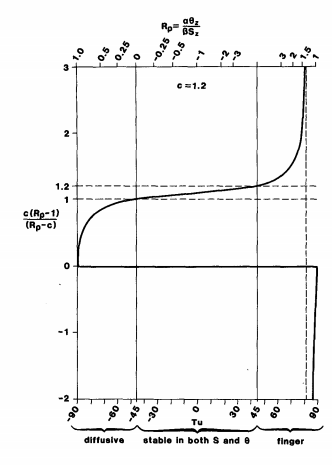
\includegraphics{mc_dougall_fig_5_graph}
    \caption{Ratio of the gradient of potential temperature on a potential density surface versus the neutral surface, as given in equation \ref{equation:gradient_ratio_theta}, plotted against values of $R_\rho$ when $c = 1.2$ \citep{McDougall1987}}
    \label{fig:gradient_theory_mcdougall_fig5_graph}
\end{figure}

\begin{figure}[htbp]
    \centering
    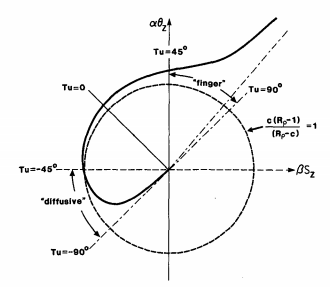
\includegraphics{mc_dougall_fig_5_turner_angle}
    \caption{Ratio of the gradient of $\theta$ on a potential density surface versus the neutral surface, as given in equation \ref{equation:gradient_ratio_theta}, plotted against values of the Turner Angle ($Tu$) when $c = 1.2$ \citep{McDougall1987}}
    \label{fig:gradient_theory_mcdougall_fig5_turner_angle}
\end{figure}

As we can see in figures \ref{fig:gradient_theory_mcdougall_fig5_graph} and \ref{fig:gradient_theory_mcdougall_fig5_turner_angle} the domain has been split into three regimes which correspond to values of $R_\rho$ and $Tu$ \citep{McDougall1987}, \citep{YOU2002}: 

\begin{enumerate}
    \item Stable in both $S$ and $\theta$: 
        \begin{itemize}
            \item $0<R_\rho$
            \item $-45^{\circ}<Tu<45^{\circ}$
            \item $\frac{c(R_\rho - 1)}{(R_\rho - c)} > 1$
        \end{itemize}
    \item Diffusive in both $S$ and $\theta$ (also known as ``double diffusive"): 
        \begin{itemize}
            \item $0<R_\rho<1$
            \item $-90^{\circ}<Tu<-45^{\circ}$
            \item $0<\frac{c(R_\rho - 1)}{(R_\rho - c)} <1$
        \end{itemize}
    \item ``Finger", where temperature is homogenised but $S$ is unstable and dominates: 
        \begin{itemize}
            \item $0>R_\rho$
            \item $45^{\circ}<Tu<90^{\circ}$
            \item $\frac{c(R_\rho - 1)}{(R_\rho - c)} >1$ or $<0$ 
        \end{itemize}
\end{enumerate}

In the two regimes ``stable" and ``finger" the ratio of the $\theta$ gradients is greater than one, suggesting that the neutral surface has the smaller gradient or ``spread" and hence is best aligned with the true mixing direction. However, in the ``double diffusive" regime the ratio of the $\theta$ gradients is between 0 and 1, suggesting that the potential density surface is best aligned with the true mixing direction. However, in \citet{McDougall1987} this analysis has only been performed for $c = 1.2$ and the gradient ratio for $\theta$. 

Theoretically we can predict what to expect by analysing the functions that calculate the gradient ratios of $\theta$ and $S$. For the following we assume that the value of $c$ is greater than zero. Under low salinity, supercooled conditions the value of $\alpha$ can be negative, but the values of salinity in the ocean mean that it is generally positive. \citep{Sverdrup1942}. Nevertheless, the case is considered in section \ref{subsection:gradienttresults} for completeness.

We can see that when $R_\rho \to \pm \infty$, $\frac{\nabla_{\sigma}\theta}{\nabla_{n}\theta}\to c$ and $\frac{\nabla_{\sigma}S}{\nabla_{n}S}\to 1$. There will be a discontinuity at $R_\rho = c$ as the denominator of both gradient ratios will be zero. 

When $R_\rho = 1$ both ratios will be 0, independent of the value of $c$. When $R_\rho = 0$ the ratios will reduce to:

\begin{equation}
    \frac{\nabla_{\sigma}\theta}{\nabla_{n}\theta} = 1 
    \label{equation:gradient_ratio_theta_R_rho_0}
\end{equation}

\begin{equation}
    \frac{\nabla_{\sigma}S}{\nabla_{n}S} = \frac{1}{c} 
    \label{equation:gradient_ratio_s_R_rho_0}
\end{equation}

Hence while the value of the gradient ratio for $\theta$ does not depend on $c$, the gradient ratio for $S$ does. If $c>1$ then both gradients will be reduced on the potential density surface in $0<R_\rho<1$. If $0<c<1$ the region where the ratios of both gradients are smaller than 1 will be $R_\rho>1$ as $R_\rho-c>0$, $R_\rho -1 >0$ and the whole expression will tend to 1 or $c$ as discussed previously.

Therefore we have identified a region where we can find a potential density surface which is better aligned to the ``true" mixing direction. If $R_\rho>0$ then we can always find a value of $c$ and therefore a potential density surface as $c$ is calculated with reference to $p_{ref}$ that performs better than the neutral surface. 

Then considering $R_\rho<0$ we can see that the value of the $\theta$ gradient ratio varies between 1 and $c$ and the value of the $S$ gradient ration varies between 1 and $1/c$. Therefore for any values of $c>0$ one gradient spread will be larger on the neutral surface and one larger on the potential density surface. This implies that the neutral surface will not be aligned with the ``true" mixing direction for $R_\rho<0$, but that neither is any potential density surface. 

Bearing this in mind three new regimes are proposed:

\begin{enumerate}
    \item Both $\theta$ and $S$ gradients smallest on neutral surface
        \begin{itemize}
            \item $R_\rho>1$ and $c>1$
            \item $0<R_\rho<1$ and $0<c<1$
        \end{itemize}
    \item $\theta$ or $S$ gradients smaller on the neutral surface but not both
         \begin{itemize}
            \item $R_\rho<0$
        \end{itemize}
    \item Both $\theta$ and $S$ gradients smallest on potential density surface
         \begin{itemize}
            \item $0<R_\rho<1$ and $c>1$
            \item $R_\rho>1$ and $0<c<1$
        \end{itemize}
\end{enumerate}

It is proposed that for $R_\rho>0$ a potential density surface can be found that is best aligned with the ``true" mixing direction by choosing the reference pressure $p_{ref}$ so that $c$ is in the required range for regime 1. For example if $R_\rho = 0.5$, we could chose $p_{ref}$ such that $c>1$. The surface that then performs best would be the potential density surface $\sigma_{p_{ref}}$.

Another way that the gradient ratio was visualised in \citet{McDougall1987} was to project the values onto a neutral density surface of interest. We can see from figure \ref{fig:gradient_Theory_mcdougall_fig_8} that we would expect the gradient of $\theta$ values to be up to 4.5 times larger on the $\sigma_0$ surface than on the neutral surface ``Nsa" in certain areas of the Atlantic basin.  

\begin{figure}[htbp]
    \centering
    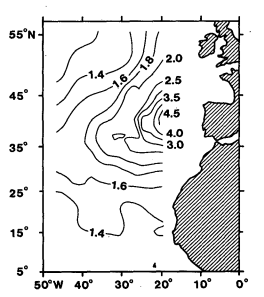
\includegraphics{mc_dougall_fig_8}
    \caption{Ratio of $\theta$ gradients on neutral surface ``Nsa" to the potential density surface $\sigma_0$ at 1500m depth, projected onto the neutral surface ``Nsa" \citep{McDougall1987}}
    \label{fig:gradient_Theory_mcdougall_fig_8}
\end{figure}

In the following sections we will compare values of the gradient ratios for $\theta$ and $S$ at different values of $R_\rho$ and $S$ in order to try and classify regimes in which we can say the neutral surface or potential density surface is best aligned with the mixing direction. We will also use ocean data taken from the \citet{WOCE2002} dataset in order to calculate values of $R_\rho$, $c$ and the two gradient ratios for $\theta$ and $S$ and project them onto various surfaces of interest. Through this we aim to understand the results given in \citet{McDougall1987} in the Atlantic region and be able to predict results in the Gibraltar Straight region. 
